<<A purely peer-to-peer version of electronic cash would allow online
payments to be sent directly from one party to another without going through a
financial institution.>>\\
Following the white paper published by the pseudonym Satoshi Nakamoto, on 31st of October 2008, Bitcoin has experienced a very rapid evolution. Many aspects of the protocol has changed in the years, permitting it to keep up with the exponential growth in terms of users, services and companies involved into it.\\
In the first place, the architecture of the network that allows the existence of Bitcoin is of type \textit{Peer-to-Peer} (P2P).\\This means that each node participating in the network is equal to the others and collaborates with the others by providing the services and functionalities defined by the shared protocol, which is executed by all nodes in a similar manner. Being the antithesis of the most well-known and widely used architecture in the current context, defined as \textit{Client/Server} (C/S), the Bitcoin network does not require centralized servers to provide any type of service. On the contrary, each node constitutes a point in the network, attributing decentralization and resilience to the protocol that only \textit{Peer-to-Peer} networks can guarantee. Examples of P2P networks that have been very successful are those used for file-sharing, initially popularized by \textit{Napster} in 1999, and later evolved into better protocols, such as \textit{BitTorrent}.\\
Similarly to the aforementioned implementations, Bitcoin was designed to be a \textit{Peer-to-Peer} system for the management and use of digital money, capable of functioning without the intervention of central authorities, with the specific goal of being an uncensorable and resilient tool against centralized control, distributed among the nodes who want to participate in the network. Due to these characteristics, the chosen design for Bitcoin could only be a P2P network.\\
In a decentralized network like Bitcoin, where there is no central authority, achieving consensus on the order and validity of transactions is crucial.\\
Another point which was an open problem before Bitcoin invention, is the so called "double-spending": it refers to the potential to spend the same bitcoin more than once, which would undermine the integrity and value of the currency.\\
To achieve the so mentioned goals, the Proof of Work (PoW) algorithm in Bitcoin was introduced. It solves the issue of consensus and prevents double-spending attacks within the blockchain network, by making it computationally expensive to tamper with the transaction history. \\
Some specialized nodes on the Bitcoin network, called miners, verify and register new transactions on the worldwide ledger. Approximately every 10 minutes, a new block is created, including the transactions that have occurred since the previous block. This process, known as mining, adds the transactions to the blockchain. Once a transaction is included in a block and added to the blockchain, it is considered confirmed, enabling the recipients of bitcoin to spend the received coins.
\begin{wrapfigure}{r}{0.5\textwidth}
\centering
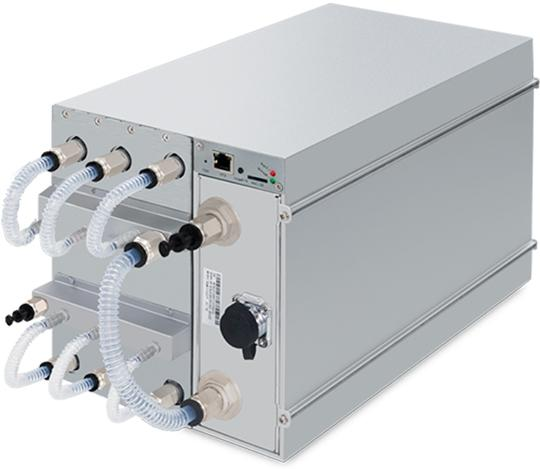
\includegraphics[width=0.35\textwidth]{Figures/bitcoin/s19xp.jpg}
\caption{Antminer S19xp hydro, one of the most powerful asic machines for Bitcoin mining}
\label{fig:antminer}
\end{wrapfigure}
The Bitcoin mining industry is highly competitive, and it experienced a significant growth in hashing power since the inception of Bitcoin. Over the years, there have been notable technological evolution. For example, in 2010 and 2011, many miners transitioned from CPU mining to GPU mining and FPGA mining, resulting in a substantial increase in hashing power. In 2013, the introduction of ASIC mining brought about another major advancement by employing specialized silicon chips designed specifically for mining, which allowed a single machine to deliver more mining power than the entire Bitcoin network in 2010.\\
In this highly competitive environment, individual miners who work alone, also known as solo miners, face slim chances of success. The probability of them finding a block to cover their expenses for electricity and hardware is extremely low, resembling a gamble akin to playing the lottery. Even the fastest consumer ASIC mining systems struggle to keep up with commercial setups that utilize tens of thousands of these chips housed in large warehouses near hydroelectric power stations. As a result, miners now join forces and form mining pools, combining their hashing power and sharing the rewards among thousands of participants. By participating in a pool, miners receive a smaller portion of the total reward but enjoy more frequent rewards, often on a daily basis, which reduces uncertainty.\\
To manage and coordinate the operations between single miners and mining pool servers, since 2010 started to appear some pooled mining protocols: Getwork, Getblocktemplate (GBT), and Stratum (V1).
The central focus of the thesis is the next generation protocol for pooled mining operations: Stratum V2. Detailed arguments about its inception, inner details, and the significant differences it brings compared to its predecessor, Stratum (V1) are analyzed in this work. \\
\begin{wrapfigure}{r}{1\textwidth}
\centering
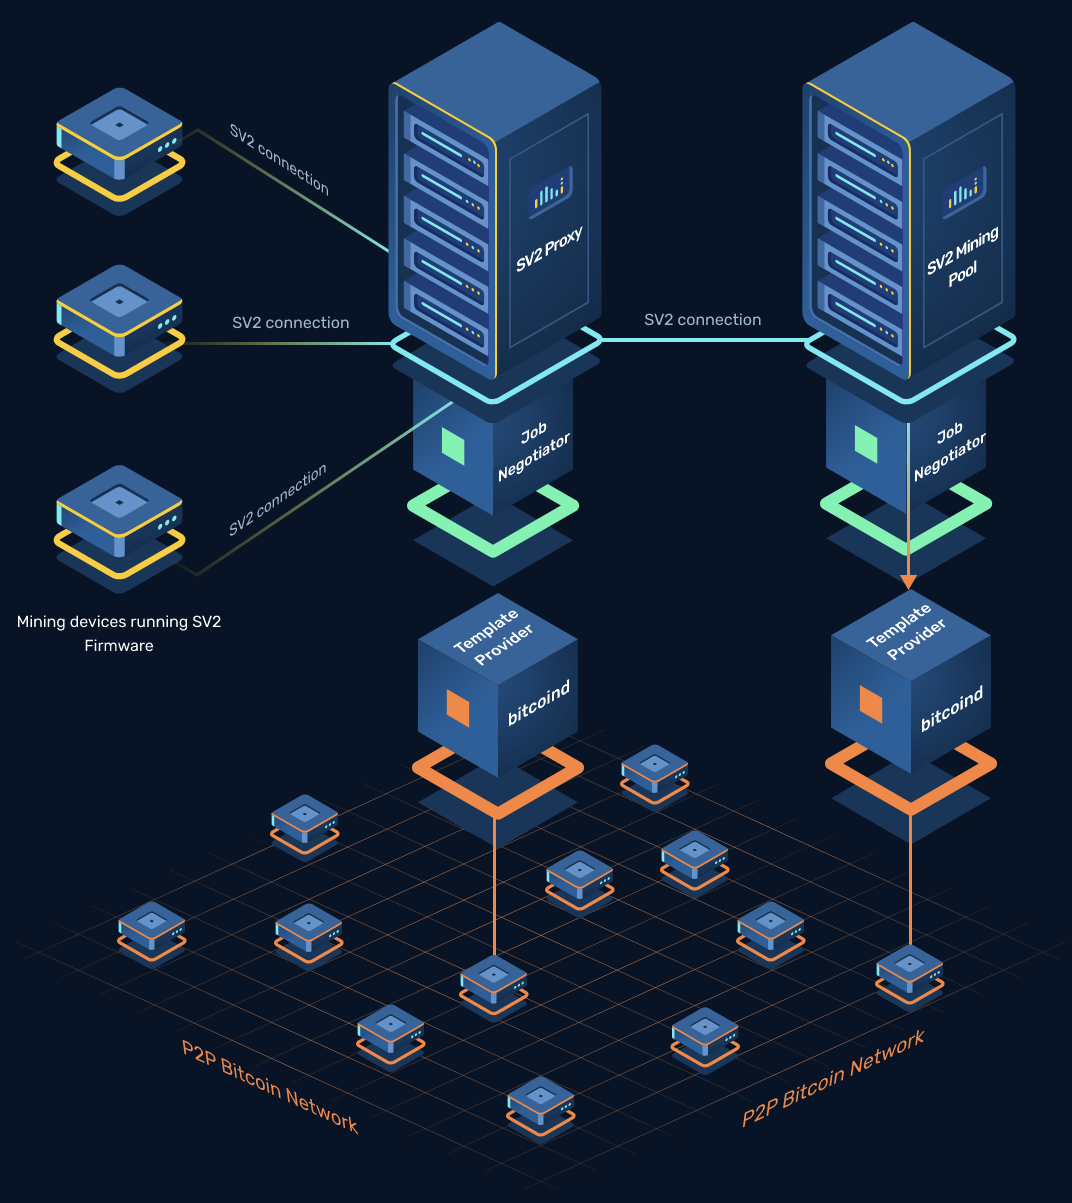
\includegraphics[width=0.65\textwidth]{Figures/sv2/sv2_9.png}
\caption{SRI configuration scheme, \href{http://stratumprotocol.org}{\textit{stratumprotocol.org}}}
\label{fig:sv2_conf}
\end{wrapfigure}
Concepts like protocol security, binary framing, and the power of transactions selection are deeply discussed, to provide to the reader all the detailed context necessary to understand the importance and the necessity of this protocol update. Additionally, the thesis presents the Stratum Reference Implementation (SRI) as a crucial resource for understanding and exploring Stratum V2. It offers detailed insights into how SRI operates, guidelines for getting started with it, and possibilities for future research and development.
Analysis of the current SRI stack is proposed, with both cpu-miner and real ASIC machines.\\
The thesis concludes by reflecting on the advancements made in Stratum V2 and their implications for the future of pooled mining in the Bitcoin ecosystem. It introduces the concept of SRI benchmarking and explores the potential of non-custodial pools as a promising avenue for future innovations.